\documentclass[DIV=calc, paper=a4, fontsize=11pt]{scrartcl}


\usepackage{makeidx}
\usepackage{graphicx}
\usepackage{flushend}

\usepackage{lmodern}
\usepackage[left=1.5cm,right=1.5cm,top=2.5cm,bottom=2cm]{geometry}
\usepackage{float}		
\bibliographystyle{plain} 
\pagestyle{plain} 
\pagenumbering{arabic}
\usepackage{fancyhdr} 	


\usepackage[T1]{fontenc}
\usepackage[utf8]{inputenc}
\usepackage[spanish]{babel}
\usepackage{hyperref}
\usepackage{graphicx}

\usepackage{lipsum}
\usepackage[protrusion=true,expansion=true]{microtype}
\usepackage{amsmath,amsfonts,amsthm}
\usepackage[svgnames]{xcolor}
\usepackage[svgnames]{xcolor}
\usepackage{booktabs}
\usepackage{fix-cm}
\usepackage{multicol}
\spanishdecimal{.}
\usepackage{siunitx}
\newenvironment{Figura}
  {\par\medskip\noindent\minipage{\linewidth}}
  {\endminipage\par\medskip}

\usepackage{sectsty}
\allsectionsfont{\usefont{OT1}{phv}{b}{n}}

\usepackage{fancyhdr}
\pagestyle{fancy}
\usepackage{lastpage}

\lhead{}
\chead{}
\rhead{}

\lfoot{}
\cfoot{}
\rfoot{\footnotesize Page \thepage\ of \pageref{LastPage}}

\renewcommand{\headrulewidth}{0.0pt}
\renewcommand{\footrulewidth}{0.4pt}

\usepackage{lettrine}
\newcommand{\initial}[1]{\lettrine[lines=3,lhang=0.3,nindent=0em]{
\color{DarkGoldenrod}{\textsf{#1}}}{}}

\usepackage{titling}

\newcommand{\HorRule}{\color{DarkGoldenrod} \rule{\linewidth}{1pt}}

\pretitle{\vspace{-120pt} \begin{flushleft} \HorRule \fontsize{22}{35} \usefont{OT1}{phv}{b}{n} \color{DarkRed} \selectfont}

\title{Filtro "pasa-bajas" pasivo\\ %Aquí va el nombre de la práctica 
Práctica 2}

\posttitle{\par\end{flushleft}\vskip 0.5em}

\preauthor{\begin{flushleft}\large \lineskip 0.5em \usefont{OT1}{phv}{b}{sl} \color{DarkRed}}

\author{García Perez Angel Yair\\
Macías Márquez Misael Iván \\
Martínez Morales Isaac David }

\postauthor{\footnotesize \usefont{OT1}{phv}{m}{sl} \color{Black}

\vspace*{0.1cm} Facultad de Ciencias, UNAM

\par\end{flushleft}\HorRule}

\date{Jueves 20 de Marzo de 2022\\Semestre 2022-1}


\begin{document}

\maketitle


\begin{abstract}
 
\textbf{Resumen:} Se midió la resistencia interna de un generador de funciones haciendo uso de un osciloscopio, un potenciómetro y el principio del divisor de voltajes, la resistencia medida fue $R_{int} = (47.34 \pm 0.02) \Omega$. También se obtuvieron los diagramas de Bode para el filtro $RC$ pasabajas y se comparó con la gráfica teórica de forma cualitativa, los diagramas obtenidos cumplieron con la tendencia esperada. Por ultimo se determinó la frecuencia de corte con valores sin incertidumbres del simulador, esta fue $f_c = 159 Hz$.


\end{abstract}

\begin{multicols}{2}




\section*{Introducción}

\subsection*{Objetivos}



\begin{enumerate}
    \item Medir la resistencia interna del generador de funciones.

    \item Obtener experimentalmente los diagramas de Bode para $v_0 (t)$, es decir,$V_0 /V_m$ vs $\omega$ y $\phi$ vs $\omega$.
    
    \item Obtener la frecuencia de corte $f_c$ (el objetivo de medir la frecuencia de corte $f_c$, con la amplitud y con el método del desfasamiento no estaba en el video de la practica por lo que no se hizo).
    
    
\end{enumerate}



\subsection*{Circuito con 2 resistencias en paralelo}
En un circuito con una fuente de voltaje y con con $2$ resistencias conectadas en paralelo, la diferencia de potencial entre la segunda resistencia esta dada por:

\begin{equation}
  V_{sal}=\frac{R}{R_{int}+R}V_{ent}  
\end{equation}

Si la diferencia de potencial $V$ es la mitad de la original:
$$V_{sal}=\frac{1}{2}V_{ent}$$
Sustituyendo se llega a que:
$$\frac{1}{2}V_{sal}=\frac{R}{R_{int}+R}V_{ent}$$
Simplificando:
$$\frac{1}{2}(R_{int}+R)=R$$
$$\iff R_{int}+R=2R$$

\begin{equation}
  \Rightarrow R_{int}=R  
\end{equation}

\subsection*{Filtro $RC$ pasabajas}

\begin{Figura}
    \centering
    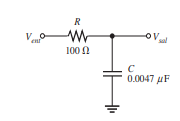
\includegraphics[width=0.9 \textwidth]{pasabajas.PNG}
    \captionof{figure}{Ejemplo de filtro $RC$ pasabajas.}
    \label{fig}
\end{Figura}

La figura 1 muestra un diagrama de bloques y una curva de respuesta general para un filtro pasabajas. El intervalo de frecuencias pasadas por un filtro dentro de límites especificados se llama banda de paso del filtro. El punto considerado como extremo superior del intervalo de la banda de paso está en la frecuencia crítica, $f_c$, como se ilustra en la figura 1.b. La frecuencia crítica ($f_c$) es la frecuencia a la cual el voltaje de salida del filtro es un 70.7\% o cuando $R\omega C = 1$ del voltaje máximo. La frecuencia crítica del filtro se conoce también como frecuencia de corte, frecuencia de ruptura, o frecuencia de 3 dB porque el voltaje de salida se encuentra a 3 dB por debajo de su valor máximo en esta frecuencia[1].

\begin{Figura}
    \centering
    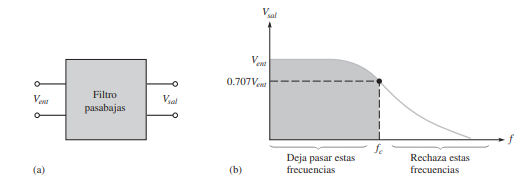
\includegraphics[width=1 \textwidth]{pasabajas1.PNG}
    \captionof{figure}{}
    \label{fig}
\end{Figura}

Cuando la entrada es de 0 Hz, el voltaje de salida es igual al voltaje de entrada porque la reactancia del capacitor  ($X_C$) es infinitamente grande. Conforme se incrementa la frecuencia de entrada, $X_C$ disminuye y, por
tanto, $V_{sal}$ disminuye gradualmente hasta que se alcanza una frecuencia a la cual $X_C=R$. Esta es
la frecuencia crítica, $f_c$, del filtro[1].

\begin{equation*}
    X_C = \frac{1}{2 \pi f_c C } = R
\end{equation*}

o bien

\begin{equation*}
    f_c = \frac{1}{2 \pi RC}
\end{equation*}

Un condensador ideal tiene una reactancia $X_C$ , que es un componente de la impedancia Z. Para una conexión en serie de resistencia y condensador el módulo de Z es[1]:

\begin{equation*}
    |Z| = \sqrt{R^2 + X_{C}^{2}}
\end{equation*}

En cualquier frecuencia, al aplicar la fórmula del divisor de voltaje, la magnitud del voltaje de salida es[1]:

\begin{equation*}
    V_{sal} = \frac{X_C}{\sqrt{R^2 + X_{C}^{2}}} V_{ent}
\end{equation*}

o bien

\begin{equation}
    \frac{V_{sal}}{V_{ent}} = \frac{X_C}{\sqrt{R^2 + X_{C}^{2}}} = \frac{1}{\sqrt{R^2 \omega^2 C^2 + 1}}
\end{equation}

\begin{Figura}
    \centering
    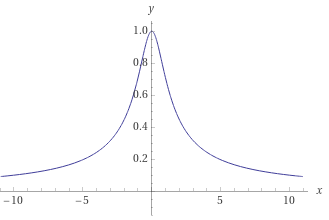
\includegraphics[width=1 \textwidth]{grafica VsVe vs frec.PNG}
    \captionof{figure}{Gráfica de la ecuación 3 que depende de $\omega$.}
    \label{fig}
\end{Figura}

Además se tiene un ángulo de fase:

\begin{equation}
    \phi = \tan^{-1} {\frac{1}{R \omega C}} - \frac{\pi}{2}
\end{equation}

\begin{Figura}
    \centering
    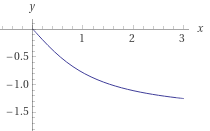
\includegraphics[width=1 \textwidth]{grafica phi vs frec.PNG}
    \captionof{figure}{Gráfica de la ecuación 4 que depende de $\omega$.}
    \label{fig}
\end{Figura}













\section*{Metodología}

\subsubsection*{PARTE I}

%\begin{Figura}
%    \centering
%    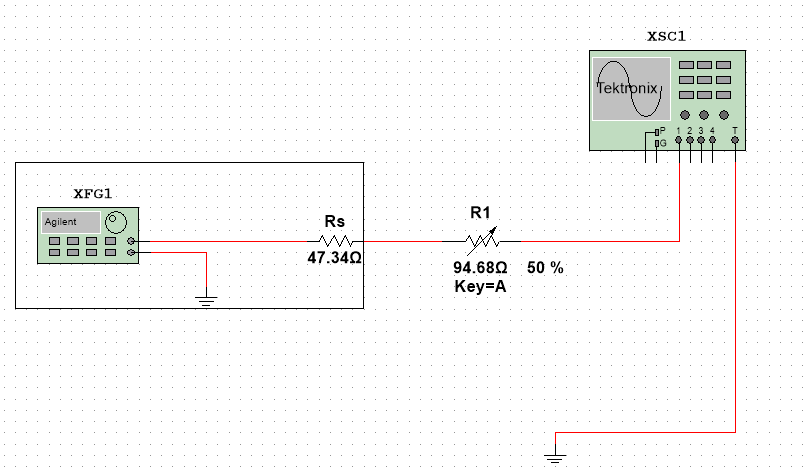
\includegraphics[width=0.9 \textwidth]{resistencia interna.PNG}
%    \captionof{figure}{Arreglo experimental: simulación en Multisim,$\mathbf{XFG1}$ generador de %funciones,  $\mathbf{R_s}$ resistencia interna del generador de funciones, $\mathbf{R_1}$ %potenciómetro 100 $\Omega$, $\mathbf{XSC1}$ osciloscopio. }
%    \label{fig}
%\end{Figura}

\begin{Figura}
    \centering
    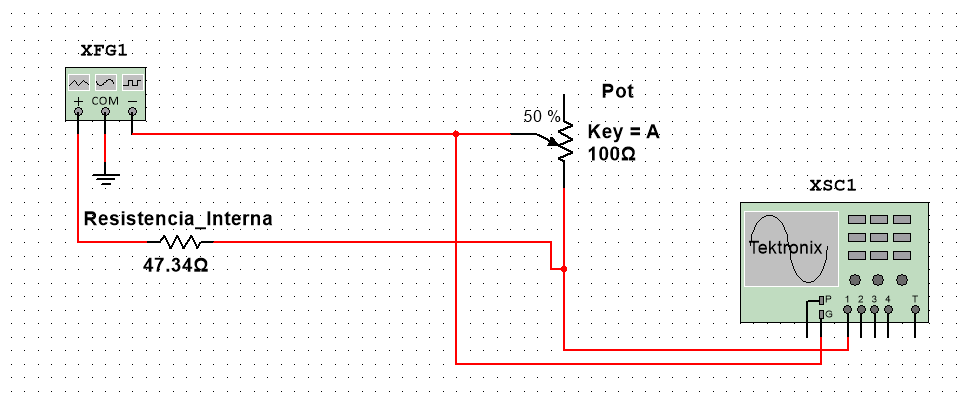
\includegraphics[width=0.9 \textwidth]{ArregloExperimentalParte1.png}
    \captionof{figure}{Arreglo experimental: simulación en Multisim,$\mathbf{XFG1}$ generador de funciones, resistencia interna del generador de funciones, potenciómetro 100 $\Omega$, $\mathbf{XSC1}$ osciloscopio.}
    \label{fig}
\end{Figura}

%\begin{Figura}
%    \centering
%    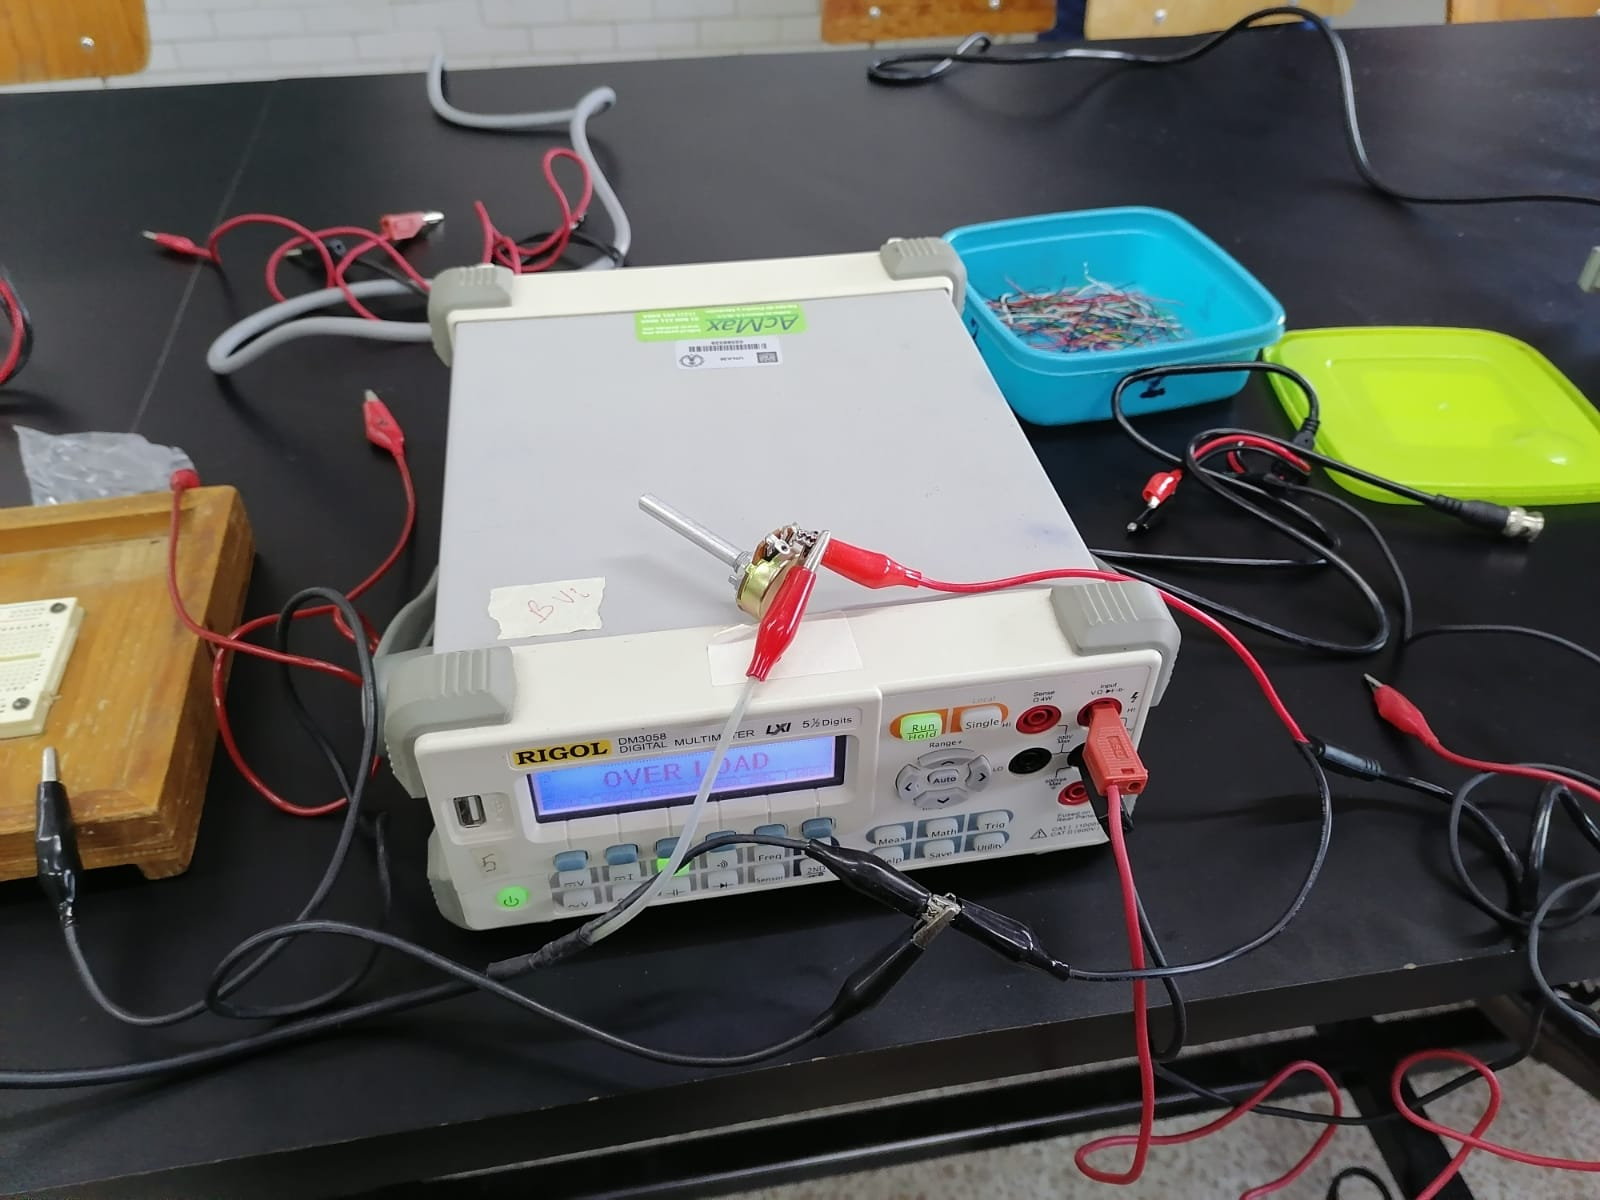
\includegraphics[width=0.9 \textwidth]{multimetro.jpg}
%    \captionof{figure}{Multimetro Rigol DM3058 digital }
%    \label{fig}
%\end{Figura}

%\begin{Figura}
%    \centering
%    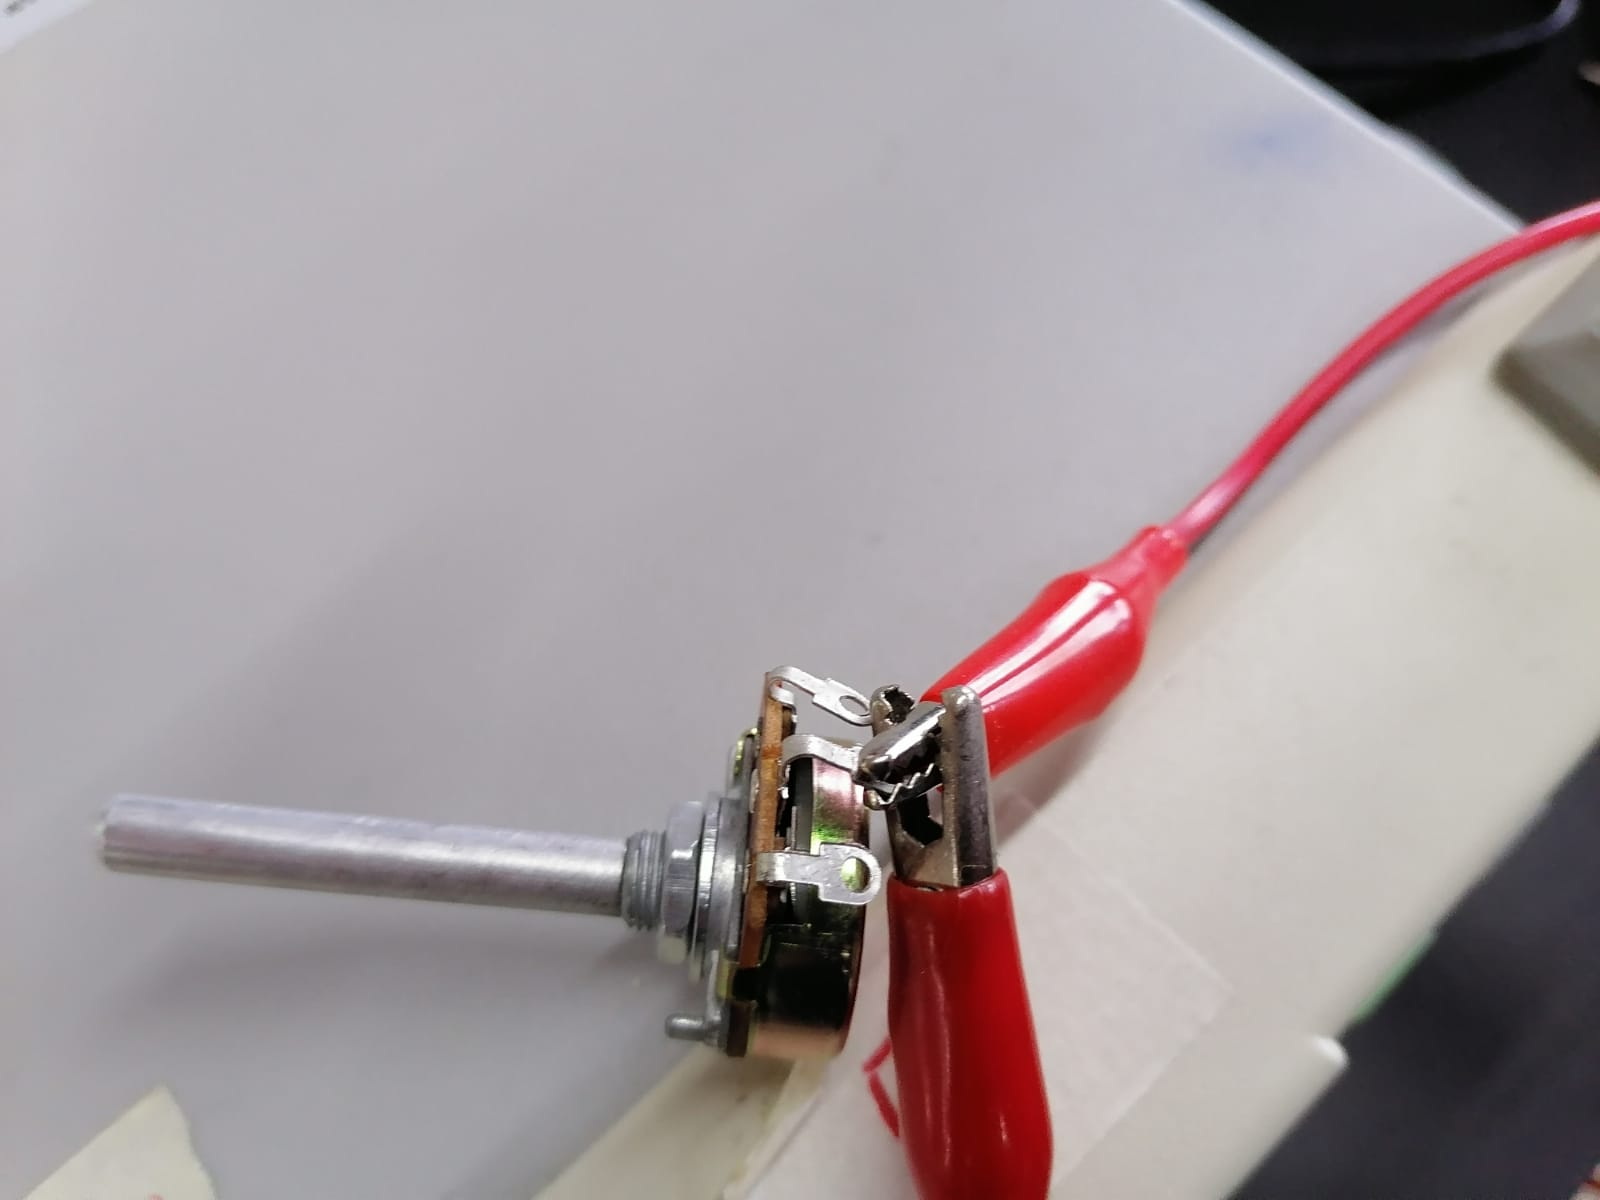
\includegraphics[width=0.9 \textwidth]{potenciometro.jpg}
%    \captionof{figure}{Potenciometro de 100 $\Omega$ }
%    \label{fig}
%\end{Figura}

%\begin{Figura}
%    \centering
%    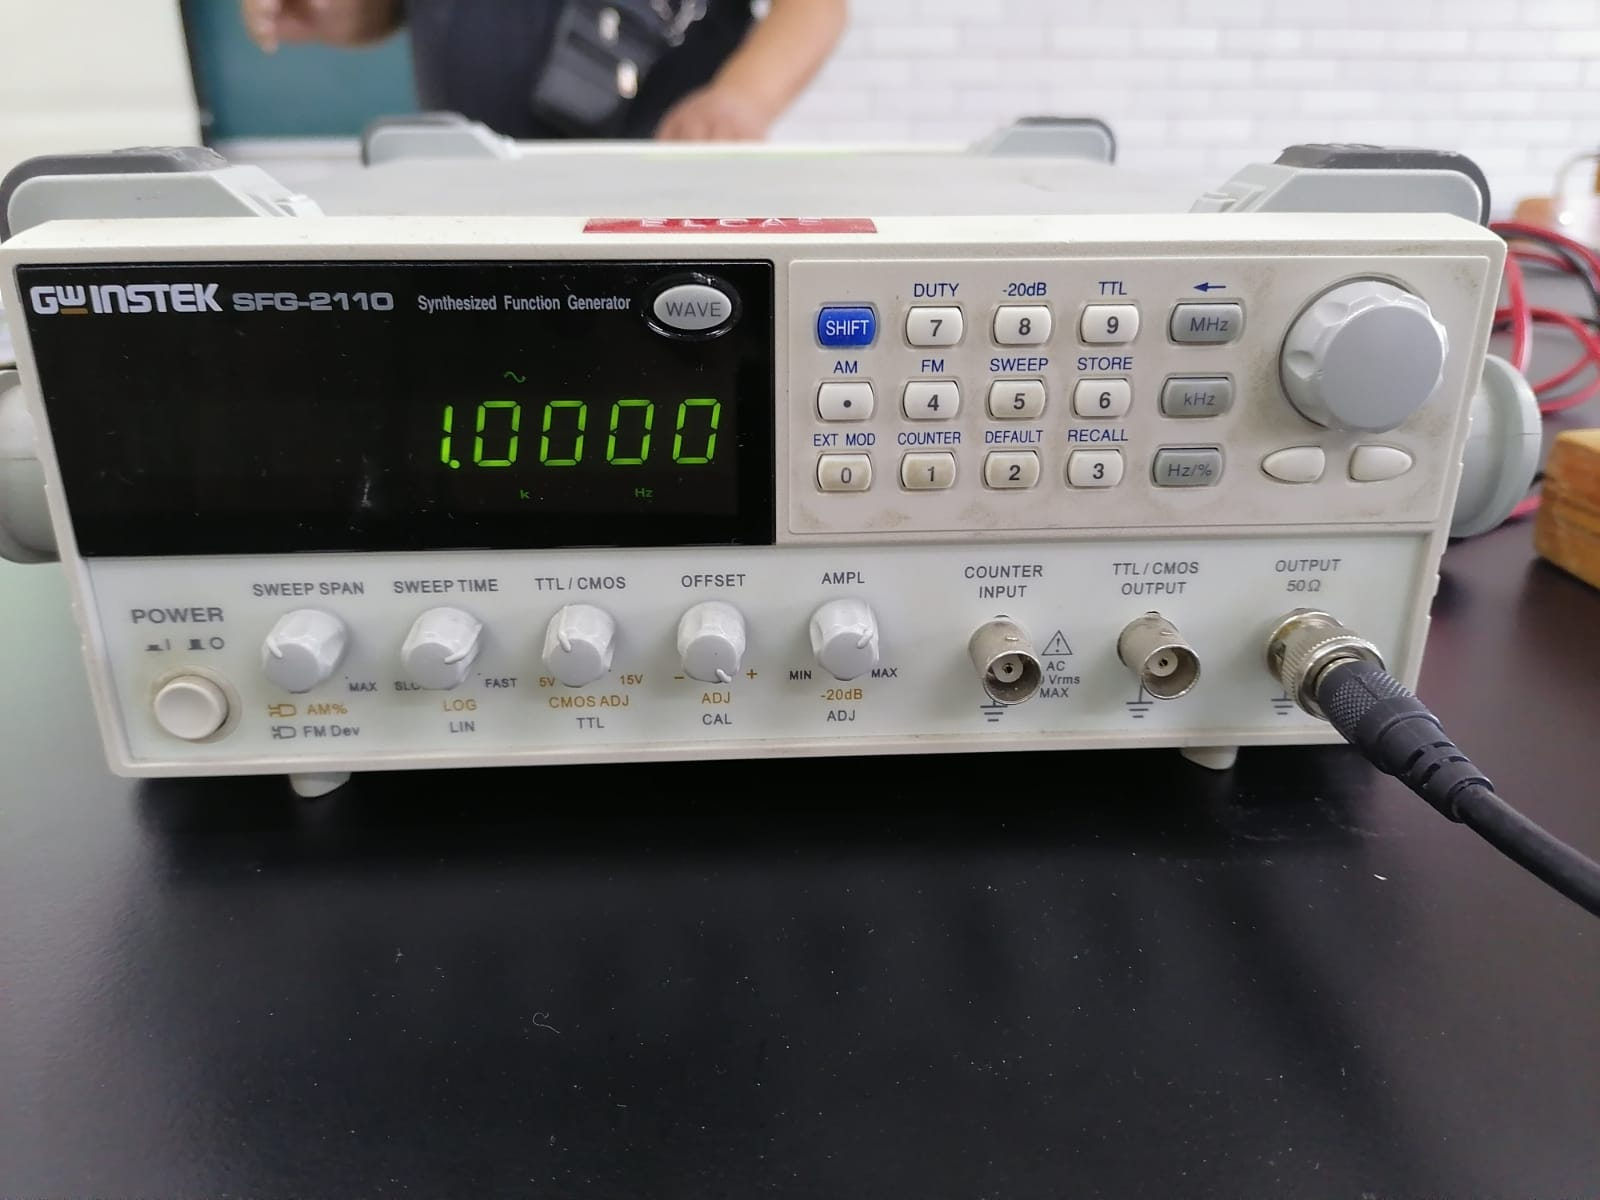
\includegraphics[width=0.9 \textwidth]{generadorfunciones.jpg}
%    \captionof{figure}{Generador de funciones GwInstek SFG-2110 con el voltaje inicial }
%    \label{fig}
%\end{Figura}

%\begin{Figura}
%    \centering
%    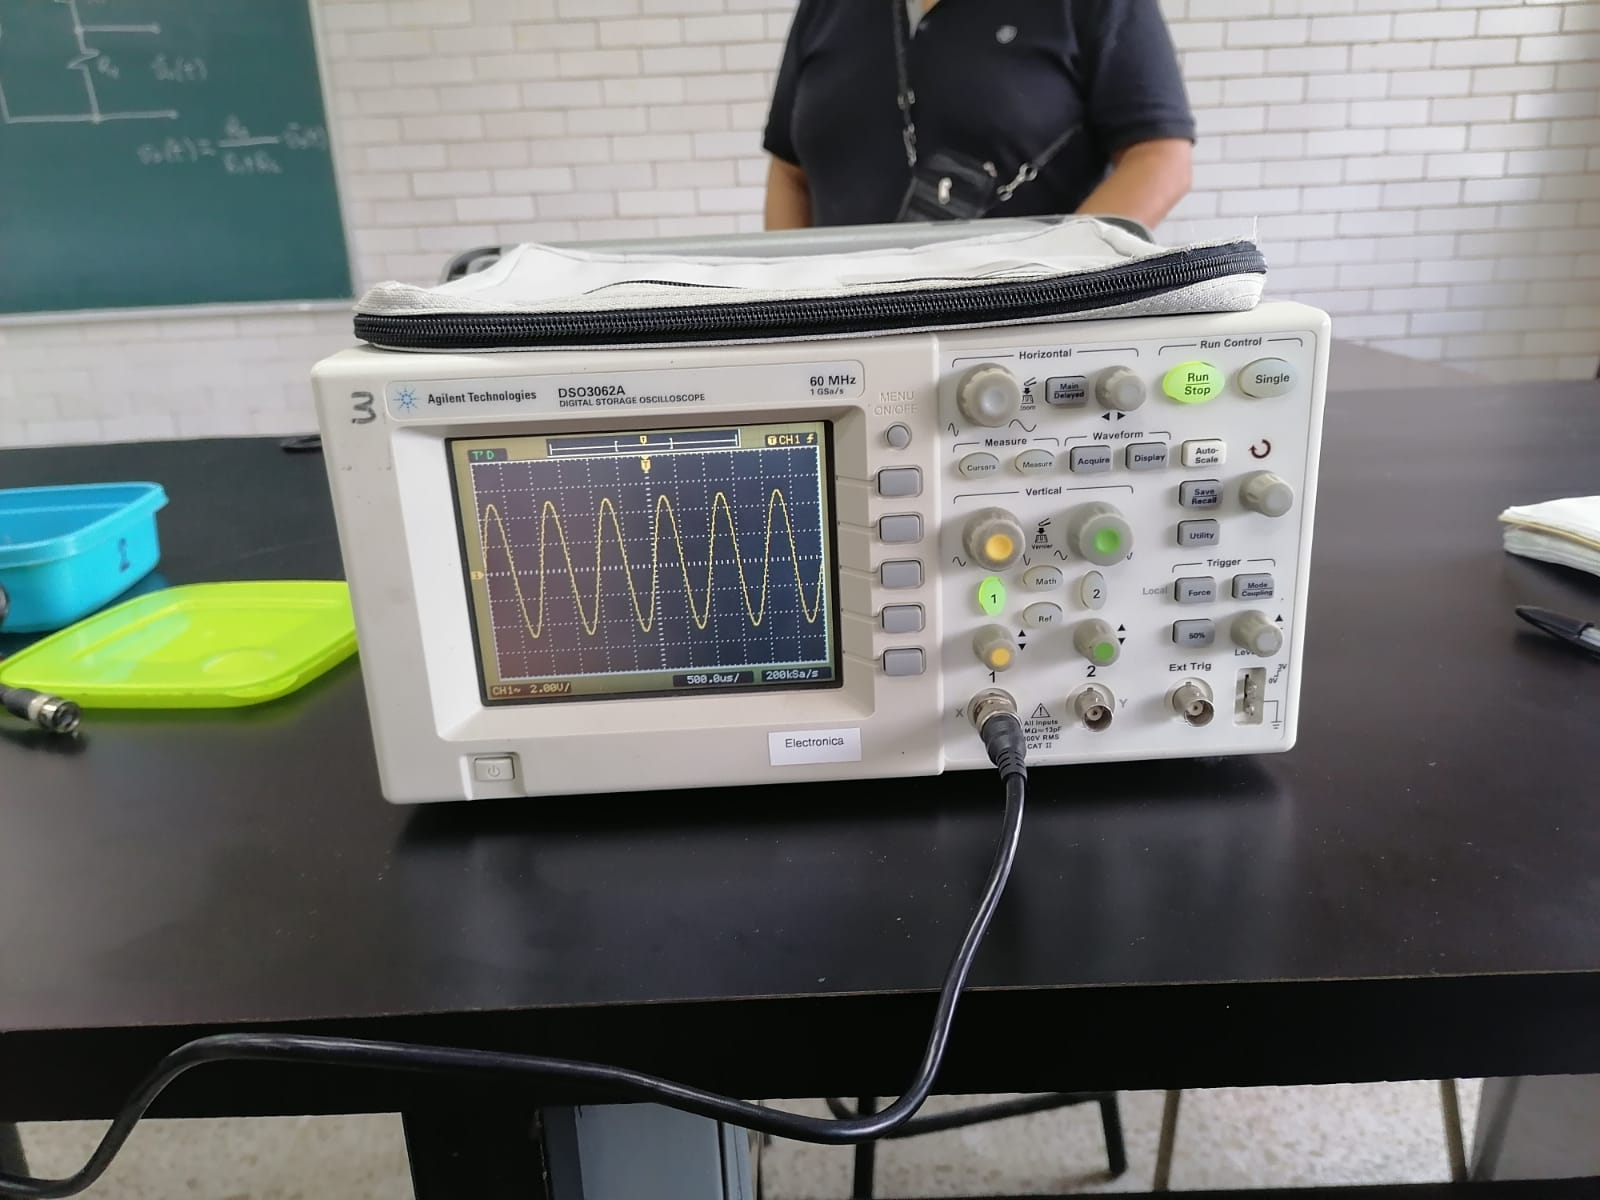
\includegraphics[width=0.9 \textwidth]{osciloscopio.jpg}
%    \captionof{figure}{Osciloscopio Agilent D50362A }
%    \label{fig}
%\end{Figura}

%\begin{Figura}
%    \centering
%    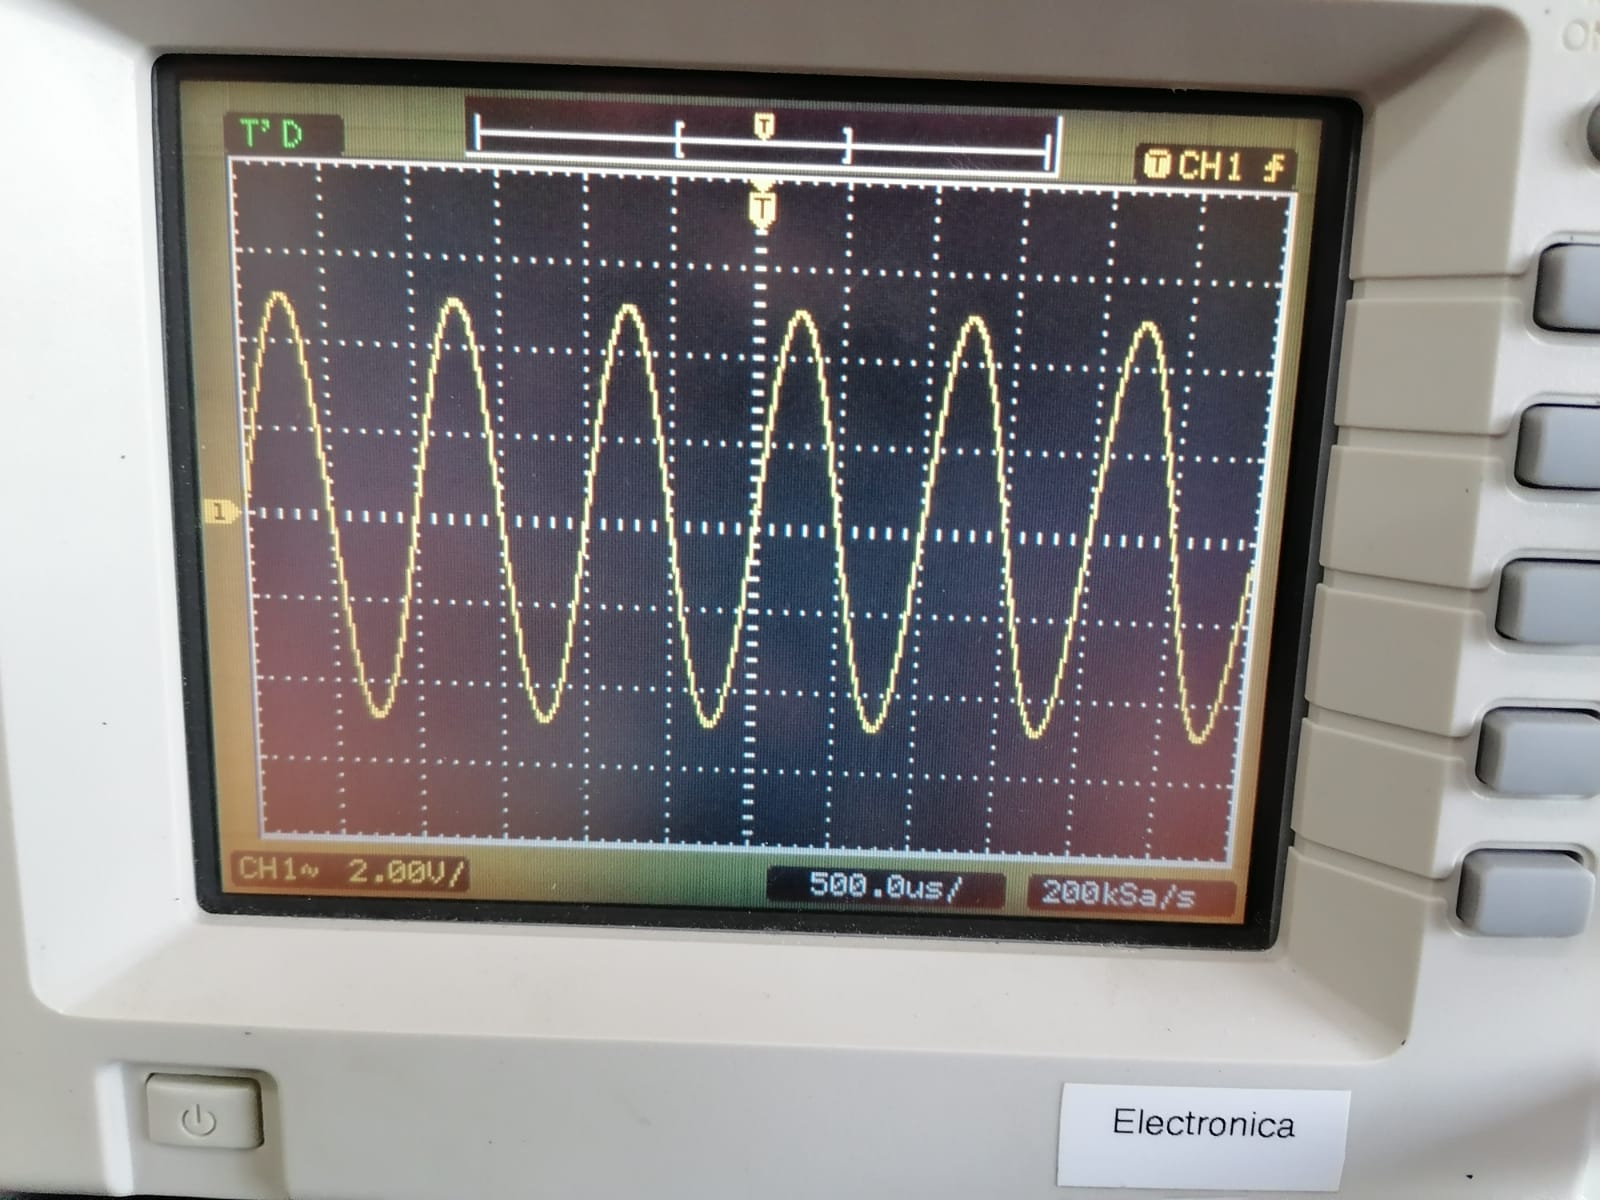
\includegraphics[width=0.9 \textwidth]{osciloscopi2.jpg}
%    \captionof{figure}{Osciloscopio con el voltaje de salida }
%    \label{fig}
%\end{Figura}


Para medir la resistencia interna del generador de funciones se utilizó un generador de funciones SFG-2110, un osciloscopio DSO3062A, un multímetro digital DM3058 y un potenciómetro de $100\Omega$
\\\\
El generador de funciones se utilizó para obtener un voltaje de $V_{ent}=10 V$, junto con su resistencia interna y con el potenciómetro se armó un circuito de tal manera que se cumpliera la ecuación 1 con $R$ la resistencia del potenciómetro, $R_{int}$ la resistencia del generador y $V_{sal}$ es el voltaje medido con ayuda del Osciloscopio.
\\\\
Para armar el circuito, debido a que la resistencia interna del generador esta adentro de este, solo se conectó la salida del generador de funciones a la terminal $1$ del potenciómetro y la terminal $2$ se conectó a la entrada del generador, con osciloscopio se midió el voltaje que había entre la terminal $1$ y la $2$.
\\\\
Después de armar el circuito se varió la resistencia del potenciómetro hasta que el valor del voltaje medido con el osciloscopio fuera la mitad del voltaje original $V_{ent}$:

\begin{equation*}
  V_{sal}=\frac{1}{2}V_{ent}  
\end{equation*}

Como vimos en la introducción, esto nos asegura que el valor de la resistencia del potenciómetro es igual al valor de la resistencia interna del generador de funciones.
\\\\
De aquí, para encontrar la resistencia interna del generador de funciones, solo basta con medir la resistencia del potenciómetro con ayuda de el multímetro.


\subsubsection*{PARTE II}

En el simulador Multisim se utilizaron osciloscopios Tektronix TD1000 ,1 generador de funciones Agilent 33120A 15MHz Function, 1 capacitor de $1 \mu F$, 2 resistencias de 47.34 $\Omega$ y $1k \Omega$. 



\begin{Figura}
    \centering
    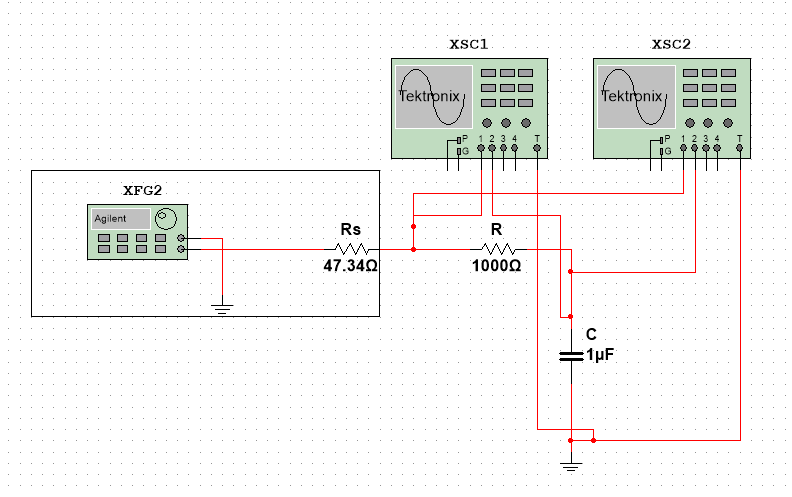
\includegraphics[width=0.9 \textwidth]{2.PNG}
    \captionof{figure}{Arreglo experimental: simulación en Multisim,$\mathbf{XSC1}$ y $\mathbf{XCS2}$ osciloscopios, $\mathbf{XFG2}$ generador de funciones, $\mathbf{R_s}$ resistencia interna del generador de funciones, $\mathbf{R}$ resistencia, $\mathbf{C}$ capacitor. }
    \label{fig}
\end{Figura}

El generador de funciones de configuró con una amplitud de $1V$ y con un rango de frecuencias de $50 Hz - 1500Hz$ pasando de 50 en 50, con el primer osciloscopio se midió la amplitud del voltaje y periodo con ayuda de la función measure, el segundo fue utilizado para medir el desfase de los voltajes obtenidos en el eje horizontal haciendo uso de los cursores y ajustando la escala de forma conveniente.






%\section*{Simulación}






\section*{Resultados y Observaciones}
\subsubsection*{PARTE I}
Después de seguir los pasos, se midió la resistencia del potenciómetro y se obtuvo que el valor de la resistencia interna es:
$$R_{int}=(47.34\pm0.02)\Omega$$
Donde la incertidumbre esta dada por:
$$\delta R_{int} = \pm((47.34)\times0.030\%+(200)\times0.005\%)\Omega$$
$$ = \pm(0.014202+0.01)\Omega$$
$$ = \pm0.024202\Omega$$

\subsection*{PARTE II}

Las mediciones de voltajes y tiempos obtenidos se pueden encontrar en una tabla en el apéndice, para calcular las incertidumbres de cada medición se utilizó el manual del instrumento usado.

\begin{equation*}
    \delta V = 3\% * \text{medición} + 0.01 * \text{medida del intervalo} + 1mV
\end{equation*}

\begin{equation*}
    \delta T = 50 ppm T = \frac{5T}{100000} 
\end{equation*}

 \begin{equation*}
     \delta \Delta t = (\text{medida del intervalo} + 100 ppm * \text{ medición} + 0.6 ns)
 \end{equation*}
 
 \begin{equation*}
    \delta f = 20 \text{ppm} f = \frac{2f}{100000} 
\end{equation*}

Para determinar la incertidumbres para el ángulo de fase y el cociente de voltajes se utilizó la regla de derivación y suma por cuadraturas de la siguiente forma:



\begin{equation*}
    \delta \left(\frac{V_{sal}}{V_{ent}}\right) = \sqrt{\left(\frac{\delta V_{sal}}{V_{ent}}\right)^2 + \left(\frac{V_{ent} \delta V_{sal}}{V_{sal}^{2}}\right)^2}
\end{equation*}



\begin{equation*}
    f_c = \frac{1}{2 \pi R C} = \frac{1}{2 \pi (1k \Omega) (1 \mu F)} = 159 Hz
\end{equation*}

\begin{Figura}
    \centering
    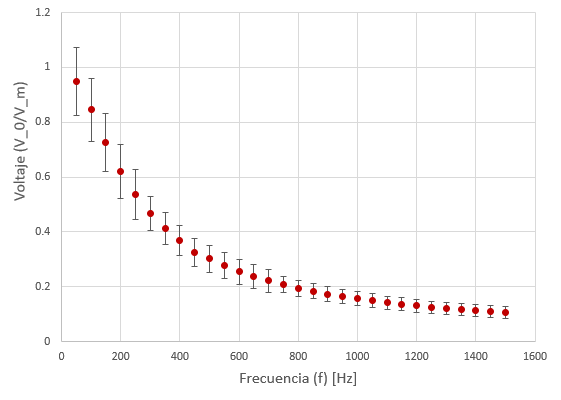
\includegraphics[width=0.8\textwidth]{grafica V.PNG}
    \captionof{figure}{Grafica $V_{sal}/V_{ent}$ vs $\omega$.}
    \label{fig}
\end{Figura}




\begin{equation*}
     \delta \phi =360^{\circ} \sqrt{\left(\frac{\delta \Delta t}{T}\right)^2 + \left(\frac{\Delta t\delta T}{T^2}\right)^2}
\end{equation*}



\begin{Figura}
    \centering
    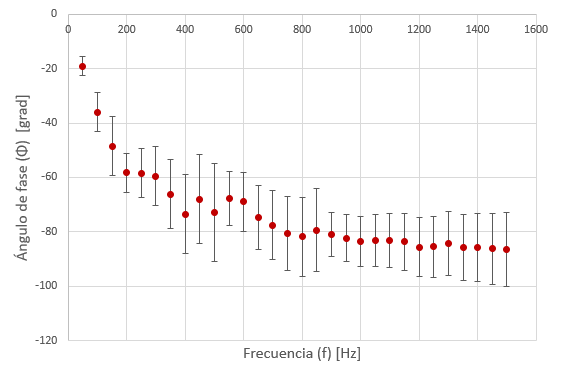
\includegraphics[width=0.8\textwidth]{grafica phi.PNG}
    \captionof{figure}{Grafica $\phi$ vs $\omega$.}
    \label{fig}
\end{Figura}











\section*{Conclusión}
El valor de la resistencia interna del generador de funciones SFG-2110 es:
$$R_{int}=(47.34\pm0.024202)\Omega$$

Los diagramas de Bode mostrados en las figuras 7 y 8 parecen cumplir con lo esperado graficado en las figuras 3 y 4.

La frecuencia de corte es:

\begin{equation*}
    f_c = 159 Hz
\end{equation*}


\begin{thebibliography}{99}

\bibitem{2} William Hart Hayt, Jack Ellsworth Kemmerly, Jamie D Phillips, and Steven M Durbin. 2019. Análisis de Circuitos En Ingeniería. Ciudad De México Mcgraw Hill Interamericana S.A. De C.V.

\bibitem{2} Floyd, Thomas L. Principios De Circuitos eléctricos (8a. Ed.). Naucalpan de Juárez: Pearson Educación, 2007. 

\end{thebibliography}

\end{multicols}



\section*{Anexos}








\subsection*{Incertidumbres para el multímetro Rigol}

\begin{Figura}
    \centering
    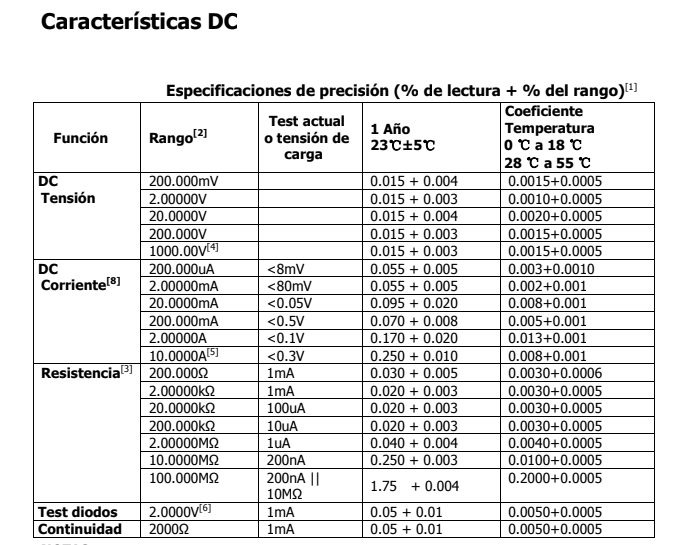
\includegraphics[width=0.6\textwidth]{incertidumbres multimetro rigol.PNG}
    \captionof{figure}{Tabla de incertidumbres para el multímetro Rigol  DM3058 digital.}
    \label{fig}
\end{Figura}



\subsection*{Incertidumbres para el osciloscopio Tektronix}

\begin{Figura}
    \centering
    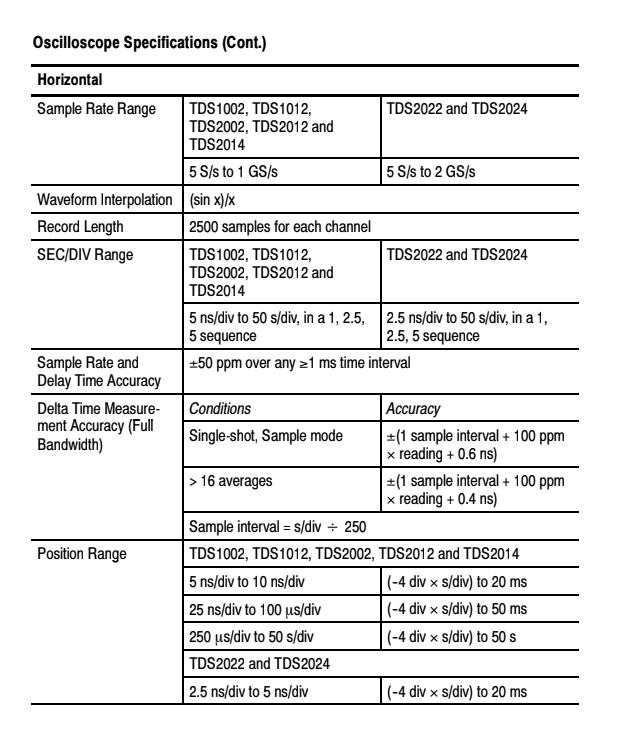
\includegraphics[width=0.6\textwidth]{incertidumbres osciloscopio tektronix 1.PNG}
    \captionof{figure}{Tabla de incertidumbres para el osciloscopio Tektronix TD1000 horizontal.}
    \label{fig}
\end{Figura}

\begin{Figura}
    \centering
    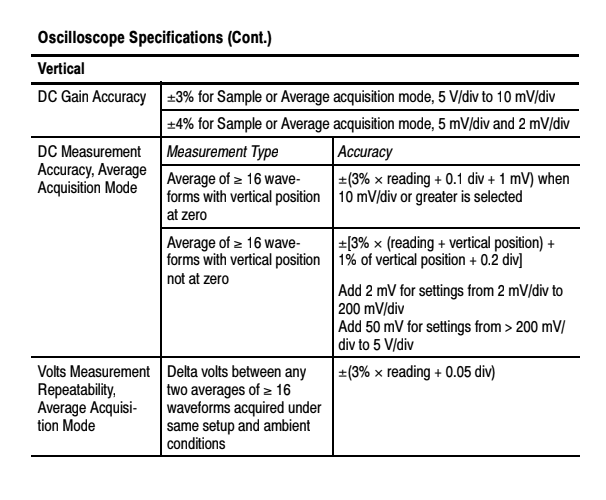
\includegraphics[width=0.6\textwidth]{incertidumbres osciloscopio tektronix 2.PNG}
    \captionof{figure}{Tabla de incertidumbres para el osciloscopio Tektronix TD1000 vertical.}
    \label{fig}
\end{Figura}

\subsection*{Incertidumbres para el generador de funciones Agilent}

\begin{Figura}
    \centering
    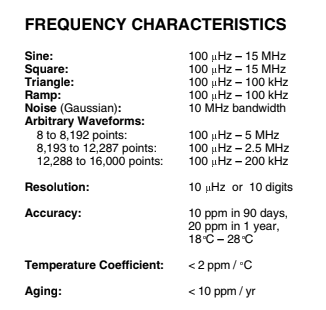
\includegraphics[width=0.6\textwidth]{incertidumbres generador de funciones agilent.PNG}
    \captionof{figure}{Tabla de incertidumbres para el osciloscopio Tektronix TD1000.}
    \label{fig}
\end{Figura}

\subsection*{Tabla de mediciones y cálculos}


\begin{Figura}
    \centering
    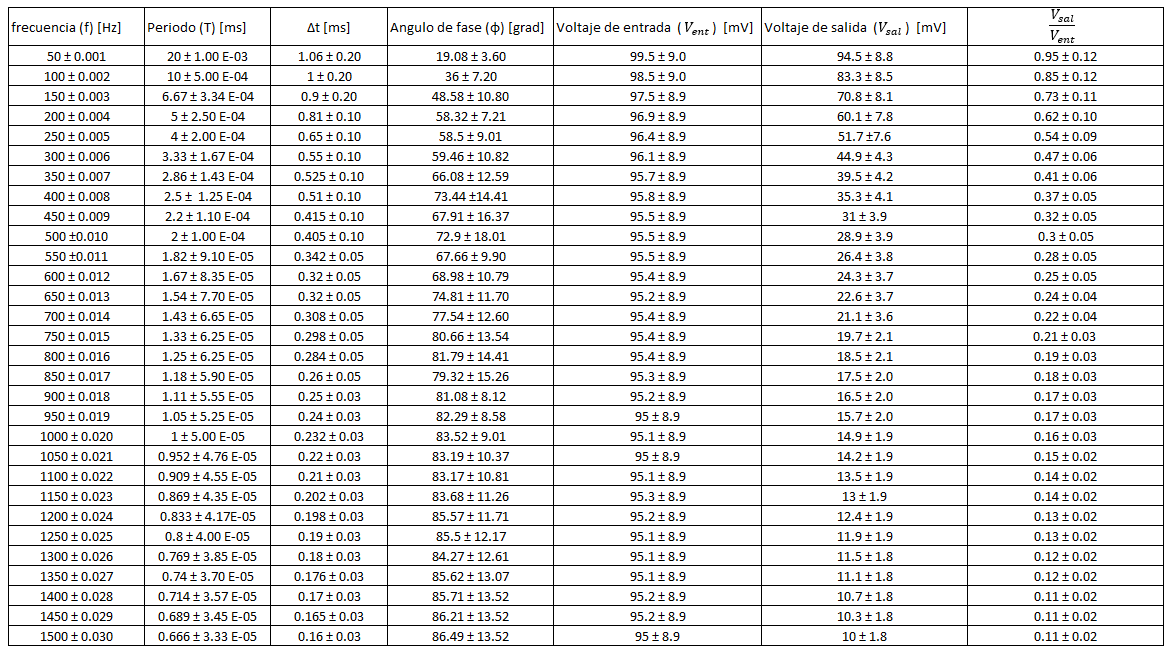
\includegraphics[width=0.8\textwidth]{tabla.PNG}
    \captionof{figure}{Tabla de mediciones y cantidades calculadas con sus incertidumbres.}
    \label{fig}
\end{Figura}




\end{document}